%-----------------------------------------------------------------------------%
\chapter{LANDASAN TEORI}
%-----------------------------------------------------------------------------%
\vspace{4.5pt}
Pada bab ini menjelaskan beberapa teori dan jurnal yang berhubungan dengan permasalahan penelitian yang digunakan pada proses penelitian.
\section{Tinjauan Pustaka}
Pembahasan mengenai teori-teori tersebut dijelaskan sebagai berikut.
\subsection{Monolit}
Monolit yaitu suatu cara untuk melakukan penyebaran. Ketika semua fungsi dalam sistem harus disebarkan secara bersama-sama, maka itu merupakan sebuah monolit.\cite{6} Monolit merupakan sebuah aplikasi perangkat lunak dimana setiap modulnya tidak bisa dieksekusi secara independen. Hal ini membuat monolit sulit digunakan pada sistem terdistribusi tanpa bantuan penggunaan \textit{frameworks} atau solusi \textit{ad hoc} seperti Objek Jaringan, \textit{RMI} atau \textit{CORBA}.
Penggunaan pada bahasa utama seperti \textit{Java},\textit{C/C++}, dan \textit{Python} pada pengembangan aplikasi di sisi \textit{server}, memiliki kemampuan dalam melakukan abstraksi untuk memecah kompleksitas program menjadi berupa modul. Namun, bahasa pemrograman ini dirancang untuk membuat \textit{artefacts} monolit. Dimana abstraksi ini tergantung pada penggunaan berbagi sumber data pada komputer yang sama (memori, database, file).[?] 


Terdapat 3 jenis monolit \cite{6}:
\begin{enumerate}[leftmargin=1.3cm]
\item \textit{Single Process Monolith}\\
Dimana sebuah kode disebarkan dengan satu proses. Setiap kode bisa berada di banyak \textit{instances} serta tempat penyimpanan dan mendapatkan data disimpan pada suatu database yang sama. Variasi lainnya yaitu modular monolit dimana setiap kode bisa bekerja secara independen tetapi perlu dijadikan satu kesatuan ketika ingin dilakukan \textit{deployment}.
\item \textit{Distributed Monolith}\\
Monolit terdistribusi adalah sistem yang terdiri dari beberapa layanan, tetapi untuk apa pun alasannya seluruh sistem harus disebarkan bersama-sama. Sebuah monolit terdistribusi bisa memiliki kesamaan dengan \textit{service-oriented architecture (SOA)}.

Monolit terdistribusi biasanya muncul  di kondisi dimana tidak cukup fokus pada konsep \textit{information hiding} dan kohesi dari fungsi bisnis. Akibatnya terbentuklah arsitektur yang memiliki kopel yang tinggi, dimana bisa perubahan menyebabkan kerusakan pada bagian sistem lain.
\item \textit{Sistem Black-Box Pihak Ketiga}\\
Aplikasi pihak ketiga merupakan sebuah monolit, misalkan sistem penggajian, sistem CRM, dan sistem SDM. Faktor umum yang terjadi yaitu aplikasi ini dibuat dan dikelola oleh orang lain dimana pengembang belum tentu memiliki kemampuan untuk mengubah kode seperti \textit{Software-as-a-Service(SaaS)}.
\end{enumerate}

Keuntungan dari Monolit:
\begin{enumerate}[leftmargin=1.3cm]
\item Sederhana dalam melakukan pengembangan karena \textit{Integrated Development Environment (IDE)} dan peralatan pengembang berfokus pada membuat satu aplikasi
\item Mudah untuk melakukan perubahan secara radikal di aplikasi. Perubahan ini bisa dari kode hingga skema database serta proses \textit{deployment}.
\item Pengujian dilakukan pada satu aplikasi, pengembang dapat membuat pengujian dari awal hingga akhir dengan lebih mudah dan terintegrasi
\item Deployment dilakukan pada satu aplikasi, pengembang hanya menyalin aplikasi dari komputer ke komputer yang lain. Dengan ini aplikasi relatif mudah dilakukan konfigurasi dan mudah diperbanyak jumlah aplikasi.
\end{enumerate}

Tantangan dari monolit:
\begin{enumerate}[leftmargin=1.3cm]
	\item Sulit dikembangkan secara berkelanjutan, karena semakin banyak orang yang bekerja pada aplikasi yang sama. Akibatnya setiap pengembang memiliki kepentingan masing-masing dalam mengelola kode yang sama dan membuat pengambilan keputusan sulit serta tidak fleksibel
	\item Memiliki reliabilitas yang rendah, karena kesalahan pada salah satu module aplikasi bisa menyebabkan kegagalan secara keseluruhan aplikasi. Akibatnya aplikasi tidak dapat digunakan oleh pengguna dan harus dilakukan deployment kembali.
	\item Tidak mudah untuk melakukan skalabilitas,setiap modul aplikasi memiliki kebutuhan sumber daya yang berbeda seperti ada module penyediaan data yang membutuhkan banyak memori sedangkan modul pemprosesan gambar membutuhkan banyak CPU, karena module ini berada pada aplikasi yang sama akibatnya pengembang harus melakukan pengorbanan pada salah satu sisi sumber daya.
	\item Terkunci pada teknologi jadul, pengembang terkunci pada teknologi awal yang digunakan untuk membangun aplikasi. Pengembang juga kesulitan ketika ingin mengadopsi teknologi baru pada aplikasi karena sangat berisiko dan sangat mahal untuk menulis kembali seluruh aplikasi antar teknologi.\\
\end{enumerate}	

\subsection{\textit{Microservice}}
\textit{Microservice} adalah beberapa \textit{service} yang bisa di deploy secara independen yang dimodelkan berdasarkan bisnis domain. \textit{Service} ini berkomunikasi satu sama lain melalui jaringan komputer dan bisa dibangun dengan berbagai macam teknologi. \textit{Microservice} adalah salah tipe dari \textit{service oriented architecture (SOA)} meskipun ada perbedaan dalam membuat batasan antara \textit{service} dan \textit{deployment} secara independen.[6]

\textit{Service} adalah komponen perangkat lunak yang memiliki kegunaannya secara khusus dimana komponen ini bisa berdiri sendiri dan secara independen dilakukan proses deployment. Service memiliki \textit{API (Application Programming Interface)} yang memberikan akses kepada \textit{client} untuk melakukan operasi. Terdapat 2 tipe operasi yaitu perintah dan kueri.[8]
\textit{API} terdiri dari perintah, kueri dan \textit{event}. Perintah dapat berupa \textit{buatPesanan()} yang melakukan aksi dan memperbarui data. Kueri dapat berupa \textit{cariPesananBerdasarkanID()} yang digunakan untuk mengambil data. \textit{Service} juga dapat membuat suatu \textit{event} seperti \textit{PesananSudahDibuat} dimana \textit{event} ini akan dikonsumsi oleh \textit{client}-nya / \textit{subscriber}.[8]

\textit{Service API} akan mengenkapsulasi internal implementasinya, sehingga pengembang aplikasi tidak bisa menuliskan kode yang melewati \textit{API}. Akibatnya arsitektur \textit{microservice} dapat mewajibkan modularitas di aplikasi.  Setiap \textit{service} di arsitektur \textit{microservice} memiliki masing-masing arsitektur sendiri dan dimungkinkan dengan teknologi yang berbeda. Tetapi kebanyakan \textit{service} memiliki arsitektur heksagonal. Dimana \textit{API} akan diimplementasi melalui adapter yang berinteraksi dengan logika bisnis[7]

Ciri Khusus \textit{Microservice}:	
\begin{enumerate}[leftmargin=1.3cm]
	\item Kecil dan berfokus pada satu hal dengan baik\\
	\textit{Service} yang dibuat memiliki \textit{encapsulation} dengan pembuatan \textit{service} dimodelkan di sekitar Domain Bisnis, tujuannya agar ketika terjadi perubahan antar \textit{service} bisa dilakukan dengan lebih mudah dan tidak berdampak pada \textit{service} lain. Oleh karena itu \textit{service} yang dibuat seminimal mungkin untuk tidak berhubungan dengan \textit{service} lain. 
	\item Otonomi / Bisa berdiri sendiri\\
	\textit{Microservice} memiliki \textit{service} yang terisolasi dimana bisa memiliki sistem operasi hingga komputer yang berbeda. Dengan ini sistem terdistribusi lebih sederhana dan nilai kopel yang rendah. Semua komunikasi antar service dilakukan melalui jaringan sehingga \textit{service} harus memiliki kemampuan di\textit{deploy} sendiri tanpa harus mempengaruhi \textit{service} lain.
	\item Data yang dikelola masing-masing \textit{service}\\
	\textit{Service} yang membutuhkan data diluar domainnya harus berkomunikasi melalui \textit{API(application programming interface)}, dengan ini setiap \textit{service} memiliki tanggung jawab terhadap datanya masing-masing sehingga data tersebut hanya bisa diubah oleh \textit{service} itu sendiri. Setiap \textit{service} memiliki data yang pribadi dan data yang bisa dibagikan kepada \textit{service} lain
\end{enumerate}	

Keuntungan dari \textit{Microservice}:
\begin{enumerate}[leftmargin=1.3cm]
	\item Memudahkan pengembangan aplikasi kompleks dan flexibel\\
	\textit{Service} berukuran kecil sehingga mudah dikelola, perubahan pada satu \textit{service} bisa diterapkan secara independen dari service lainnya. Bila terjadi kegagalan di satu \textit{service} tidak berdampak besar pada \textit{service} lainnya karena \textit{service} masing-masing terisolasi selain itu proses pemulihan bisa dilakukan dengan mudah dan cepat.
	\item Bisa dilakukan skaling secara independen\\ 
	Setiap \textit{service} memiliki fungsi yang berfokus pada satu hal,  dimana setiap \textit{service} bisa memiliki kebutuhan sumber daya berbeda. Penggunaan sumber daya ini bisa dikelola dengan mudah dan cepat karena setiap service dapat di\textit{deploy} dengan jumlah \textit{service} yang berbeda.
	\item Mudah melakukan percobaan dan penggunaan teknologi baru\\
	Arsitektur \textit{microservice} mengeliminasi komitmen penggunaan secara lama pada suatu teknologi. Dengan ini pengembang dapat memilih berbagai teknologi dalam membangun \textit{service} serta \textit{service} yang kecil dan berfokus lebih mudah untuk dilakukan migrasi antara teknologi yang berbeda. 
\end{enumerate}	

Tantangan dari \textit{Microservice}:
\begin{enumerate}[leftmargin=1.3cm]
	\item Menemukan \textit{service} yang tepat itu sulit\\
	Salah satu tantang terbesar dari membuat \textit{microservice} yaitu tidak adanya cara yang pasti bagaimana untuk melakukan dekomposisi dengan baik. Dimana \textit{service} yang didekomposisi dengan tepat tidak mudah ditemukan dan bila dilakukan dengan tidak benar dapat sebaliknya membuat \textit{distributed monolith}. 
	\item Memiliki kompleksitas karena merupakan suatu terdistribusi\\
	Setiap \textit{service} untuk berkomunikasi antar \textit{service} memiliki tantangan masing-masing seperti latensi, konsistensi data, dan kondisi ketika beberapa \textit{service} mengalami kegagalan. \textit{Microservice} juga meningkatkan kompleksitas operasional oleh karena itu untuk melakukan \textit{deployment} sebaiknya menggunakan proses otomatisasi.
	\item \textit{Deployment} yang melibatkan beberapa service\\
	Untuk melakukan \textit{deployment} ini dibutuhkan koordinasi antara tim pengembang \textit{servic} ketika menambahkan atau mengubah fitur yang berdampak pada beberapa \textit{service} maka dari itu harus dibuat perencanaan \textit{deployment} berdasarkan ketergantungan antar \textit{service}.
\end{enumerate}	

Pola \textit{Microservice}:
\begin{center}
	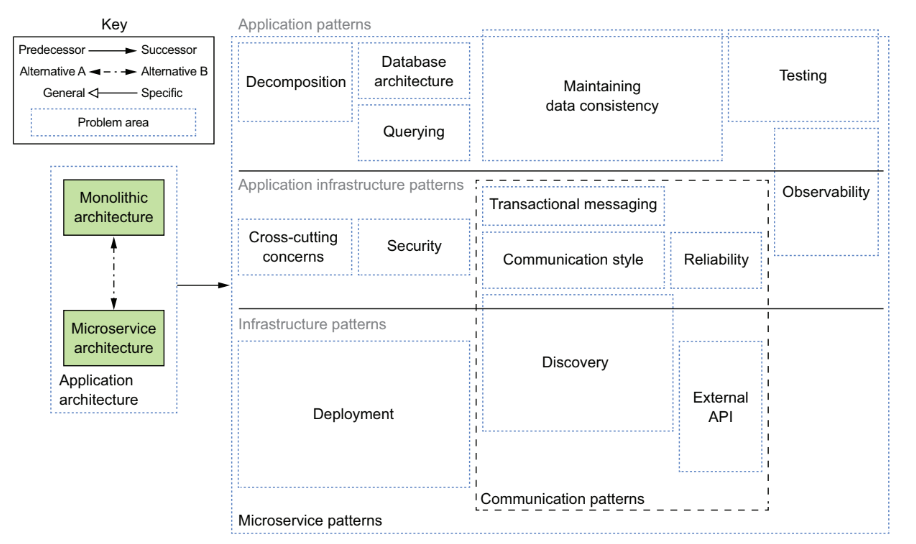
\includegraphics[width=12cm]{img/PolaMicroservice.png}
	\captionof{figure}{
	Pola dalam menyelesaikan masalah di arsitektur \textit{Microservice} \cite{8} }
	\label{fig:msa}
\end{center}
\begin{enumerate}[leftmargin=1.3cm]
	\item \textit{Application patterns}
	Permasalahan yang harus diselesaikan oleh pengembang aplikasi
	- Proses kueri
	- Dekomposisi aplikasi menjadi service
	- Menjaga data konsistensi dan implementasi proses transaksi
	- Mengotomatiskan proses pengujian  service
	\item \textit{Application infrastructure} 
	Permasalah infrastruktur yang memiliki pengaruh pada proses pengembangan aplikasi
	- Pola komunikasi
	- Pola mengatasi permasalahan antar service
	\item \textit{Infrastructure patterns} 
	Permasalahan infrastruktur yang muncul diluar dari pengembangan aplikasi
	- Pola Komunikasi
	- Pola Service Deployment
	- Pola observability untuk mengetahui bagaimana aplikasi bekerja\\	
\end{enumerate}	

\subsection{\textit{Enterprise Resource Planning}}
\textit{Enterprise Resource Planning} (ERP) adalah suatu sistem perangkat lunak yang memungkinkan perusahaan untuk mengotomatisasikan dan mengintegrasikan proses bisnisnya dengan komputerisasi. Dengan ini setiap informasi yang diperlukan di proses bisnis dapat dibagikan dan digunakan disemua bagian perusahaan dengan alur terstruktur. Sistem ERP dapat mengeliminasi duplikasi data dan memberikan integrasi data. Sistem ERP memiliki database dimana semua transaksi bisnis dapat direkam, diproses, dipantau dan dilaporkan. Tujuannya agar proses bisnis bisa dilakukan dengan lebih cepat, murah, dan transparan \cite{1}.

Sistem ERP dapat memberikan dukungan untuk proses bisnis perusahaan melalui modul yang terpisah. Setiap modul adalah aplikasi perangkat lunak yang dibangun khusus untuk setiap operasi bisnis. Umumnya modul yang ditemukan pada ERP yaitu Modul Produksi, Modul Manajemen Rantai Pasokan, Modul Keuangan, Modul Penjualan \& Pemasaran, Modul Sumber Daya Manusia, dan modul pelengkap lainnya seperti \textit{e-commerce} \cite{1}.

Arsitektur ERP \cite{1}: 
\begin{enumerate}[leftmargin=1.3cm]
	\item \textit{The Tiered}\\
	Arsitektur \textit{tiered} umumnya dirancang dalam bentuk lapisan yang didasarkan dari model \textit{client-server} atau bisa disebut \textit{N-Tier}. Dalam arsitektur ini setiap komponen ERP disusun kedalam masing lapisan seperti lapisan \textit{user interface}, lapisan aplikasi dan lapisan \textit{database} / penyimpanan data.
	\item \textit{Web-based}\\
	Arsitektur \textit{Web-based} mengadopsi teknologi berorientasi objek web dimana pengguna yang ingin menggunakan sistem ERP bisa mengakses melalui \textit{browser} dan internet. \textit{Object-oriented technology} diimplementasi untuk mencampur data dan fungsi yang tersedia di berbagai web \textit{service}.
	\item \textit{Service Oriented}\\
	\textit{SOA(Service Oriented Architecture)} adalah sistem yang dimana terdapat fungsi  modular yang berkomunikasi melalui jaringan. Satu atau lebih \textit{service} bisa berkordinasi dalam suatu aktivitas fungsi bisnis. 
	\item \textit{Cloud}\\
	\textit{Cloud} dapat memberikan solusi bagi organisasi ketika mengadopsi sistem ERP pada kegiatan bisnisnya. Sistem ERP dengan arsitektur \textit{cloud} bisa dikategorikan sebagai tipe \textit{SaaS(Software as a Service)}. Organisasi akan membayar pihak ke tiga setiap periode berdasarkan modul yang digunakannya.\\ 
\end{enumerate}

\subsection{Analisis Kode}
Analisis Kode adalah suatu proses mengekstraksi informasi mengenai suatu program dari kode atau artifak. Proses ini bisa dilakukan secara manual yaitu dengan melihat kode program atau bahasa mesin namun kompleksitas program yang tinggi membuat proses secara manual sangat sulit dan tidak efektif. Sehingga diperlukan alat otomatisasi yang dapat membantu proses analisis kode. Alat ini dapat memberikan informasi kepada pengembang mengenai program yang dianalisis.[9] 

Anatomi Analisis Kode:
\begin{enumerate}[leftmargin=1.3cm]
	\item Ekstraksi Data\\
	Proses ini adalah proses pertama kali dilakukan sebelum melakukan analisis kode, data yang diekstrasi berasal dari kode program. Umumnya dilakukan dengan \textit{syntatic analyzer} atau \textit{parser}. Proses \textit{Parser} ini mengkonversi urutan karakter menjadi suatu kata-kata dan mengekstraksi nilai semantik sebenarnya. Tujuannya agar memudahkan proses analisis/transformasi dan penambahan data lainnya.
	\item Representasi Informasi\\
	Proses yang merepresentasikan informasi kode menjadi bentuk yang lebih abstrak. Tujuan dari fase ini untuk membentuk beberapa bagian kode agar terhubung pada analisis secara otomatis. Representasi ini kebanyakan berupa graph seperti \textit{Abstract Syntax Trees (AST)}, \textit{Control Flow Graphs (CFG)}, dan \textit{Call Graph}.
	\item Eksplorasi Pengetahuan\\
	Setelah informasi direpresentasikan, informasi dibuat menjadi suatu kesimpulan. Kesimpulan bisa dibuat secara kuantitatif atau kualitatif, proses visualisasi penting dalam proses eksplorasi pengetahuan kode program.
\end{enumerate}

Strategi Analisis Kode:
\begin{enumerate}[leftmargin=1.3cm]
	\item Statik vs Dinamis\\
	Analisis secara statik menganalisis program tanpa dieksekusi untuk mendapatkan semua informasi yang kemungkinan akan dieksekusi. Sedangkan secara Dinamis, program mengumpulkan informasi yang dieksekusi dengan nilai yang diberikan. Beberapa teknik analisis menggabungkan kedua pendekatan ini.
	\item \textit{Sound vs Unsound}\\
	\textit{Sound} yaitu analisis yang bisa menjamin secara keseluruhan dan kebenaran eksekusi program. Sedangkan \textit{Unsound} tidak bisa secara keseluruhan menjaminkan kebenaran hasil analisis program. Namun dalam banyak kasus analisis \textit{Unsound} memiliki hasil yang benar selain itu memiliki kelebihan yaitu mudah diimplementasi dan efisien.
	\item \textit{Flow sensitive vs Flow insensitive}\\
	\textit{Flow sensitive} memperhatikan dan menyimpan urutan proses eksekusi sedangkan \textit{Flow insensitive} tidak memperhatikan urutan proses eksekusi sehingga tidak memiliki informasi ketergantungan pada suatu proses dan hanya dapat menyatakan proses tersebut ada.
	\item \textit{Context sensitive vs Context insensitive}\\
	\textit{Context in-sensitive} hanya menghasilkan satu hasil yang berhubungan dalam semua konteks. Sedangkan \textit{context sensitive} memiliki hasil berbeda ketika konteks berbeda. Pendekatan ini bertujuan untuk menganalisis proses pembuatan analisis umumnya tanpa adanya informasi mengenai konteks yang akan digunakan. \textit{Context sensitive} penting untuk menganalisis program modern dimana terdapat suatu abstraksi.
\end{enumerate}

Tantangan Kode Analisis:
\begin{enumerate}[leftmargin=1.3cm]
	\item Perbedaan bahasa kode program\\
	Banyak peningkatan dan perubahan pada bahasa pemrograman seperti \textit{dynamic class loading} dan \textit{reflection}. Konsep ini juga terdapat pada proses pengubahan tipe data, \textit{pointer}, \textit{Anonymous types} yang membuat proses \textit{parser} sulit. Fitur pada pemrograman ini meningkatkan fleksibilitas ketika program berjalan dan membutuhkan analisis secara dinamik yang lebih kuat.
	\item \textit{Multi-Language}\\
	Banyak aplikasi yang dibuat sekarang dibangun dengan berbagai bahasa pemrograman. Dimana sekarang perlengkapan pembuatan aplikasi masih belum bisa menganalisis secara keseluruhan pada aplikasi yang menggunakan banyak bahasa pemrograman. Seperti aplikasi berbasis web yang memiliki \textit{HTML}, \textit{ASP}, \textit{Java} dan lainnya.
	\item Analisis secara \textit{Real-Time}\\
	Analisis ini dapat memberikan keuntungan bagi pengembang karena memberikan informasi tambahan selama pengembang membuat aplikasi seperti \textit{code coverage} dan analisis kebocoran memori. Proses analisis juga kerap kali membutuhkan penggunaan sumber daya komputasi yang tinggi dan memori yang banyak.\\
\end{enumerate}

\subsection{\textit{Clustering}}
\textit{Clustering} yaitu suatu proses untuk melakukan pengelompok atau klasifikasi objek. Objek bisa ditentukan dari pengukuran atau berdasarkan hubungan antar objek lainnya. Tujuan dari clustering yaitu untuk  menemukan struktur data yang valid. Cluster terdiri dari sejumlah object serupa yang dikumpulkan / dikelompokan bersama.[10]

Metode \textit{Clustering} yang umumnya digunakan:
\begin{enumerate}[leftmargin=1.3cm]
	\item \textit{Hierarchical Clustering} \\
	Metode \textit{Hierarchical Clustering} adalah sebuah prosedur untuk mentranformasi sebuah \textit{proximity matrix} menjadi beberapa partisi. Clustering adalah sebuah partisi dimana komponen dari partisi disebut \textit{clusters}. Beberapa partisi memiliki suatu urutan dan tingkatan berdasarkan bagaimana partisi tersebut disatukan. Terdapat 2 pendekatan algoritma dalam membentuk suatu partisi yaitu secara \textit{agglomerative} dan \textit{divisive}. 
	Pendekatan \textit{Agglomerative} dimulai dari setiap objek memiliki partisi masing-masing dan terpisah, kemudian algoritma mengukur nilai \textit{proximity matrix} setiap objek untuk menentukan berapa banyak penggabungan partisi lain yang perlu dilakukan. Proses dilakukan berulangkali dan jumlah partisi akan berkurang hingga tersisa satu partisi, satu partisi ini memiliki keseluruhan objek. Sedangkan pendekatan secara \textit{divisive} melakukan hal yang sama seperti \textit{Agglomerative} namun prosesnya terbalik yaitu dimulai dari satu partisi.
	\item \textit{Partitional Clustering} \\
	\textit{Partitional} menggunakan pendekatan dimana diberikan sejumlah \textit{n} pola pada data dimensional, kemudian tentukan partisi dari pola menjadi beberapa cluster. Pendekatan \textit{Hierarchical} populer digunakan dibidang biologi, sosial, dan ilmu perilaku karena keperluan untum membentuk suatu taxonomi. Sedangkan \textit{Partitional} digunakan umumnya di aplikasi teknik. 
	
	Dimana satu partisi lebih penting, Metode \textit{Partitional} juga memiliki efisiensi dan kompresi yang cocok untuk data yang besar sehingga pola dalam cluster memiliki kemiripan satu sama lain daripada pola dalam \textit{cluster} yang berbeda. Pemilihan nilai \textit{cluster} bisa ditentukan secara opsional, kriteria \textit{cluster} yang valid harus ditentukan seperti \textit{square-error} untuk menentukan apakah partisi yang dibuat optimal. Kriterianya sendiri bisa dibagi menjadi secara global atau lokal.  

\end{enumerate}	
Pemilihan Partisi :	
\begin{enumerate}[leftmargin=1.3cm]
	\item Secara Struktural dan Perilaku dari \textit{microservice}
	\item Nilai \textit{Coupling} dan \textit{Cohesion}
	\item Berdasarkan ketergantungan data antar \textit{Class}
\end{enumerate}	

\subsection{Dekomposisi}
Pemilihan bagian yang ingin didekomposisi untuk menjadi Service:[6]
\begin{enumerate}[leftmargin=1.3cm]
	\item Proses bisnis
	\item Sub-domain (DDD)
	\item Analisis Kode
\end{enumerate}	

Pola untuk Proses Dekomposisi:
\begin{enumerate}[leftmargin=1.3cm]
	\item Pola Strangle 
	\item Pola UI Composition
	\item Branch By Abstraction
	\item Parallel Run
	\item Decorating Collaborator
	\item Change Data Capture
\end{enumerate}	

Tantangan dan Hambatan Dekomposisi:
\begin{enumerate}[leftmargin=1.3cm]
	\item Latensi Jaringan
	\item Menjaga konsistensi data antar service
	\item Adanya God Class yang mencegah dekomposisi
\end{enumerate}	

\subsection{Teknologi dan \textit{Library}}
\subsubsection{\textit{Docker}}
...
\subsubsection{\textit{gRPC}}
...
\subsubsection{\textit{PyCG}}

\section{Tinjauan Studi}
\par Pada Tabel \ref{tbl:StateoftheArt} diberikan penjelasan mengenai studi terkait dalam penelitian:

\begingroup
\setlength{\LTleft}{-20cm plus -1fill}
\setlength{\LTright}{\LTleft}
\begin{small}
	\begin{longtable}{|p{3cm}|p{3.5cm}|p{3cm}|p{3.5cm}|}
		\caption{\textit{State of the Art}}\\
		\hline
		\textbf{Jurnal} & \textbf{Rumusan Masalah} & \textbf{Metode} & \textbf{Hasil}\\
		\endfirsthead
		\hline
		Munezero Immaculée Josélyne, Doreen Tuheirwe-Mukasa, Benjamin Kanagwa, and Joseph Balikuddembe. (2018, May). "Partitioning microservices: a domain engineering approach." \cite{11} &
		... &
		... &
		... 
		\\
		
		\hline
		Tyszberowicz, S., Heinrich, R., Liu, B., Liu, Z. (2018). "Identifying Microservices Using Functional Decomposition." \cite{12}  & 
		... &
		... &
	    ... 
		\\

		\hline
		Khaled Sellami, Mohamed Aymen Saied, and Ali Ouni. (2022). "A Hierarchical
		DBSCAN Method for Extracting Microservices from Monolithic Applications" \cite{13} &
		... &
	    ... &
		... 
		\\
		
		\hline
		Shanshan Li, He Zhang, Zijia Jia, Zheng Li, Cheng Zhang, Jiaqi Li, Qiuya Gao, Jidong Ge, Zhihao Shan. (2019). "A dataflow-driven approach to identifying microservices from monolithic applications."  \cite{14} &		  
		... &
		... &
		... 
		\\

		\label{tbl:StateoftheArt}\\

		\hline
		Chaitanya K. Rudrabhatla. (2020). "Impacts of Decomposition Techniques on Performance and Latency of Microservices."  \cite{3} &
		... &
		... &
		... 
		\\
		
	\end{longtable}
\end{small}
\endgroup
Pada penelitian Munezero Immaculée Josélyne, kendala yang muncul ketika membuat  microservice yaitu bagaimana mengetahui batasan antara komponen service. Dengan menggunakan Domain Driven Design bisa memberikan beberapa cara untuk mengetahui batasan pada domain yang besar dan kompleks. Metode Domain Driven Design direkomendasikan dalam proses perancangan microservice. \\

Kemudian penelitian yang menggunakan pendekatan secara functional dilakukan dari mengidentifikasi microservice dengan spesifikasi use-case dari software requirements. Kemudian melakukan dekomposisi melalui tool visualisasi dimana visualisasi dihasilkan dari relasi antar objek, operasi dan variabel yang berasal dari source code.
Selain itu ada pendekatan dengan menggunakan pengelompokan khusus menggunakan hierarchical clustering yang dikombinasi dengan struktur dan analisis semantic. Dengan ini bisa mendeteksi outlier. Hasil dari pengelompokan akan dikomparasi dan dilakukan evaluasi.\\

Pendekatan dataflow-driven juga dapat membuat identifikasi secara sistematik dan mudah dipahami dalam melakukan dekomposisi dibandingkan dengan cara manual lainnya. Proses yang dilakukan yaitu dimulai dari menggunakan Use Case Specification dan Logic Bisnis dan kemudian diubah menjadi Data Flow diagram. Hasil dari diagram ini akan memberikan kandidat microservice yang bisa dibuat.\\

Penelitian lainnya berfokus pada dampak dari pendekatan masing-masing dekomposisi karena bila dekomposisi tidak dilakukan dengan baik maka bisa terjadi permasalah pada latensi, kompleksitas dan ketidakefisienan. Penelitian ini menggunakan skenario e-commerce pada aplikasi microservice yang didekomposisi dengan pendekatan yang berbeda.\\

\section{Tinjauan Objek}
Pada bagian ini akan dijelaskan mengenai objek dan aplikasi terkait yang akan digunakan dalam tugas akhir ini. Object yang digunakan adalah sebuah aplikasi Enterprise Resource Planning yang di deploy secara monolit, yaitu Odoo.\\

Odoo merupakan aplikasi bisnis open source yang dapat mencakup semua kebutuhan perusahaan seperti CRM(Customer Relationship Management), eCommerce, akuntansi, inventaris, POS(Point of Sales), manajemen proyek dan lainnya. Aplikasi ini flexibel karena bisa dikembangkan lebih lanjut bila diperlukan dan bisa diubah karena memiliki lisensi source code yang terbuka. \\

Arsitektur yang digunakan pada Odoo yaitu three-tier arsitektur dimana tampilan, aturan bisnis dan tempat penyimpanan data memiliki lapisan terpisah. Dengan tujuan memudahkan dan mempercepat pengembang untuk melakukan modifikasi aplikasi tanpa harus mengganggu lapisan lainnya.\\

\begin{center}
	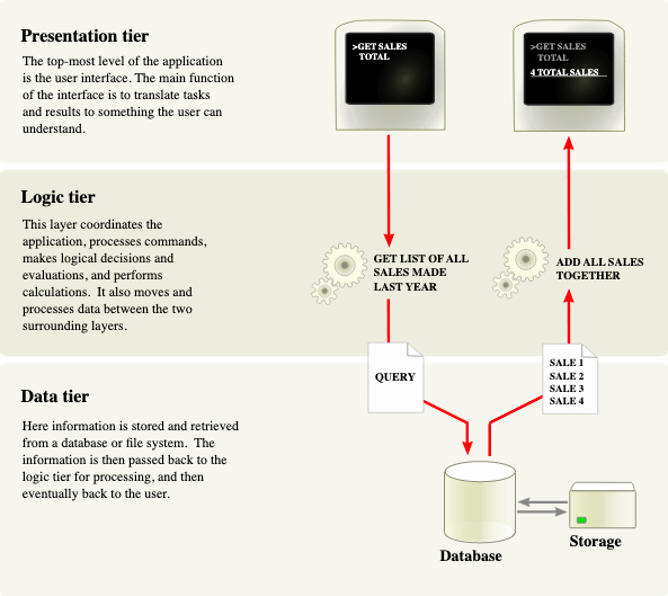
\includegraphics[width=12cm]{img/arsitekturOdoo.PNG}
	\captionof{figure}{Ilustrasi Arsitektur Odoo}
	\label{fig:asd}
\end{center}

Pada tingkatan paling atas yaitu tampilan(presentation tier), tampilan ini yang akan berinteraksi langsung dengan pengguna yang menggunakan aplikasi. Tampilan ini dibangun dengan teknologi web yaitu HTML5, Javascript, dan CSS. Tingkatan dibawahnya yaitu aturan bisnis(logic tier) yang berisi instruksi yang memproses data dan memberikan tanggapan dari interaksi kepada pengguna. Aturan pada Odoo hanya ditulis dalam bahasa pemrograman Python. Sedangkan pada tingkat paling bawah adalah tempat penyimpanan menggunakan DBMS(Database Management System), Odoo hanya bisa mendukung database PostgreSQL.\\

Odoo memiliki struktur kode yang dibentuk sebagai module untuk setiap fiturnya. Sehingga dari sisi server dan client memiliki hubungan yang disatukan menjadi satu paket tersendiri. Dimana module adalah koleksi dari fungsi dan data untuk menyelesaikan satu tujuan. Modul pada Odoo bisa ditambahkan, diganti, diubah untuk menyesuaikan kebutuhan bisnis. Dimana pada pengguna module dilambangkan dengan nama Apps, tetapi tidak semua module adalah Apps. Modules juga bisa direfrensikan sebagai addons.\\

\begingroup
\setlength{\LTleft}{-20cm plus -1fill}
\setlength{\LTright}{\LTleft}
\begin{small}
	\begin{longtable}{|p{3cm}|p{5cm}|p{5cm}|}
		\caption{Komposisi dari Module pada aplikasi Odoo}\\
		\hline
		\textbf{Elemen} & \textbf{Keterangan} & \textbf{Contoh}\\
		\endfirsthead
		
		\hline
		    Business Objects
		  & Object yang akan digunakan di module dimana setiap attribute secara otomatik dipetakan ke kolom database dengan ORM
		  & File python yang memiliki class\\
		\hline  
		Objects Views
		  & Menangani bagaimana data ditampilkan di pengguna. Seperti visualisasi form, list, kanban dan lainnya
		  & Berupa file XML dengan struktur yang sudah ditentukan Odoo\\
		\hline
		Data Files
		  & Mengelola bagaimana model data seperti laporan, konfigurasi data, data contoh dan lainnya
		  & Berupa file XML atau CSV\\
		\hline
		Web Controllers
		  & Menangani permintaan dari browser/client
		  & File python yang memiliki class namun merupakan turunan dari class odoo.http.Controller\\
		\hline
		  Static Web Data
		  & File yang digunakan hanya ditampilkan kepada client di website
		  & File gambar, File CSS, dan File JavaScript\\
		 \hline  
	\end{longtable}
\end{small}
\endgroup

Struktur database yang dibentuk pada konfigurasi umum di Odoo memiliki jumlah tabel ±566 tabel, tabel ini merupakan keseluruhan dari aplikasi dimana dapat diidentifikasi 31 tabel utama yang digunakan pada aplikasi. Berikut adalah diagram dari database yang dibuat dengan alat DBeaver Visualize, dengan attribute hanya sebuah key dari tabel. \\
\begin{center}
	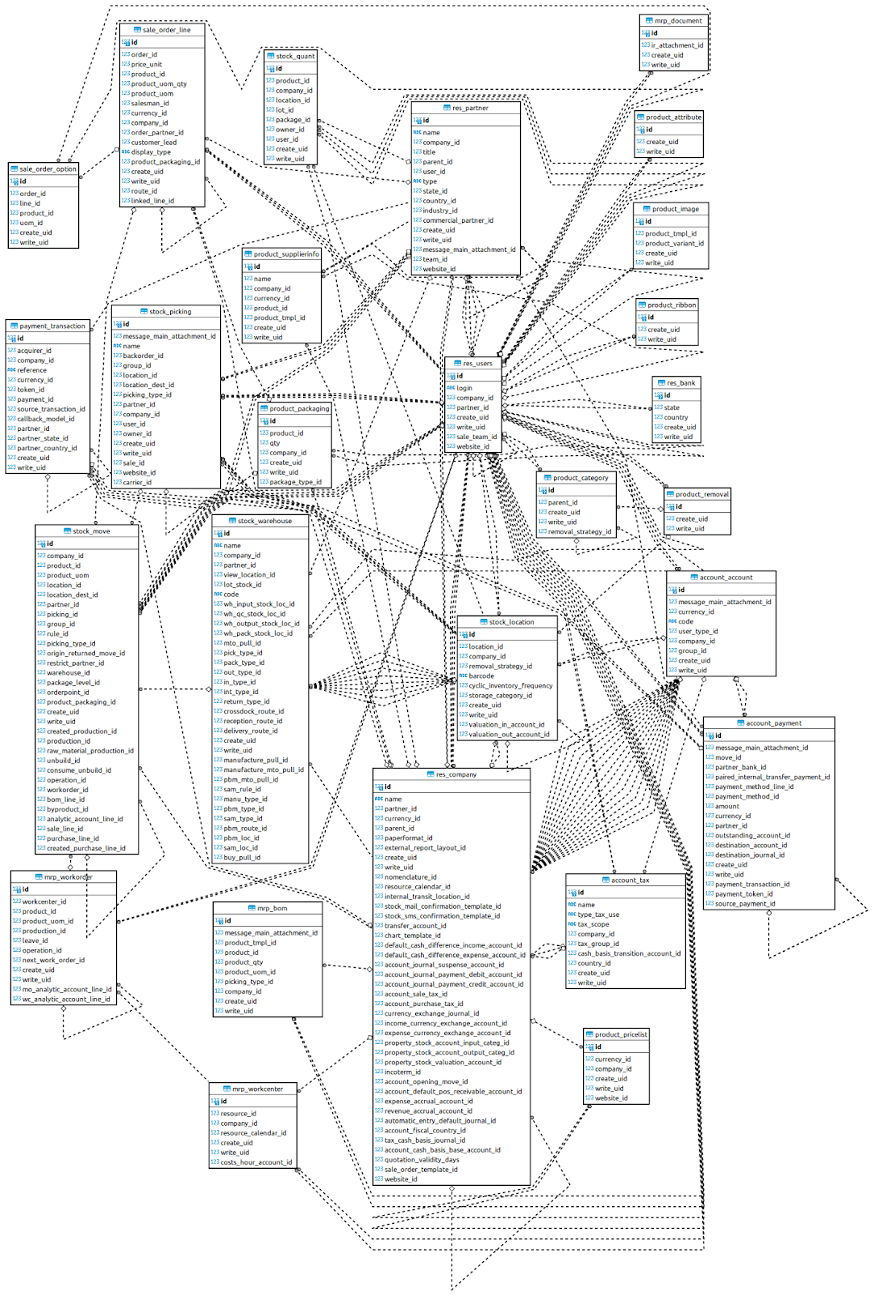
\includegraphics[width=14cm]{img/DatabaseOdoo.png}
	\captionof{figure}{Diagram Database Odoo}
	\label{fig:asd}
\end{center}



